		
\documentclass{beamer}

% Setup appearance:

%\usetheme{Darmstadt}
\usetheme{Marburg} 
%\usetheme{Goettingen}
\useinnertheme{rounded}
%\usecolortheme{beaver}
%\usefonttheme{serif}
%\usefonttheme[onlylarge]{structurebold}
%\setbeamerfont*{frametitle}{size=\normalsize,series=\bfseries}
\setbeamertemplate{navigation symbols}{}
%\usecolortheme{rose} %para que aparezcan los blocks eviroments
%\useoutertheme{infolines} 

\usepackage[spanish]{babel}
\usepackage[latin1]{inputenc}
\usepackage{times}
\usepackage[T1]{fontenc}
\usepackage{amsmath}
\usepackage{mathtools}
\usepackage{calrsfs}
%\usepackage{graphicx}
\usepackage{hyperref}

% Setup TikZ

\usepackage{tikz}
\usetikzlibrary{arrows}
\tikzstyle{block}=[draw opacity=0.7,line width=1.4cm]

\title[] 
{%
  Introducci�n a POSIX\\ 
 %5ta ESE - Horco Molle 2015 %
}
	
\author[]
{
Bioing.~Juan~Manuel Reta \\ Mgt Eduardo Filomena~\
}

%\insertshortdate
\date[2015]
{}

\begin{document}

\begin{frame}
% \begin{center}

%\end{center}
  \titlepage
\begin{center}
  
	
\includegraphics[height=1cm]{Imagenes/logo_ruse}
\hspace{1cm}
	
\includegraphics[height=1cm]{Imagenes/acse}
\end{center}

\end{frame}



%\end{frame}
\section{Historia}

%\begin{frame}{}
%\includegraphics[height=2cm]{Imagenes/3d_printer3}
%\includegraphics[height=2cm]{Imagenes/application3}

%\end{frame}
\begin{frame}{De UNIX a POSIX}

%\begin{block}{De UNIX a POSIX}
\begin{columns}
\column{.6\textwidth}

En 1973 Unix comenz� a reescribirse en el recientemente desarrollado lenguaje C. Esto supon�a no tener que preocuparse de las peculiaridades del procesador de la m�quina subyacente.
\column{.4\textwidth}

\begin{figure}
	\centering
		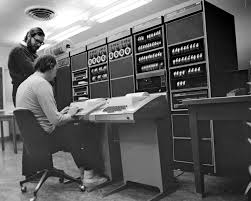
\includegraphics[height=3cm]{./Imagenes/unix}
	\label{fig:unix}
\end{figure}
\end{columns}
\vspace{.5cm}
 Se hac�a muy sencillo modificar el sistema operativo o portarlo a otras arquitecturas. \\
 \vspace{.5cm}
El desarrollo de Unix se divide en ramas: 

\begin{itemize}
\item AT\&T introduc�a su Unix System 3.
\item La universidad de Berkeley desarrollaba el BSD
v4.
\item Interactive Systems, Microsoft o Human Computer Resources distribu�an versiones adaptadas a ordenadores m�s modestos.
\end{itemize} 

%\end{block}


\end{frame}


\begin{frame}{POSIX}

\begin{columns}
\column{.6\textwidth}

Surgi� entonces la necesidad de crear pautas generales de manera que los distintos \textit{sabores} de Unix que hab�an surgido fuesen compatibles entre s�. Es lo que m�s tarde se conocer� como el est�ndar POSIX.

\column{.4\textwidth}

\begin{figure}
	\centering
		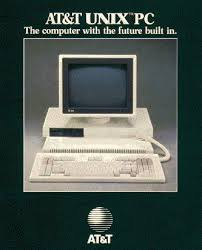
\includegraphics[height=3cm]{./Imagenes/att}
	\label{fig:att}
\end{figure}
\end{columns}
\vspace{.3cm}

En 1980 la organizaci�n \textit{/user/group} forma un comit� para la redacci�n de un est�ndar que especifique la interfaz entre el programador y el sistema operativo.
\begin{itemize}
\item Independizarse de las versi�n de Unix desarrolladas hasta el momento, buscando que se pudiesen crear aplicaciones o sistemas operativos, sin tener que comprar los productos de un solo distribuidor.
\item Definici�n clara y no ambigua de la interfaz entre el sistema operativo y el usuario.
\end{itemize} 


\end{frame}
\section{Est�ndar}
\begin{frame}{POSIX.1}

En 1984 el priemr borrador fue enviado al Comit� t�cnico de Sistemas Operativos (TCOS-SS) de la IEEE.\\
En Abril de 1986, la IEEE hizo public� el primer borrador del estandar y en 1988 se public� la versi�n difinitiva del \textbf{POSIX.1 - IEEE 1003.1-1988.}\\
 
\begin{itemize}
\item \textbf{POSIX.2:} Estandarizaci�n de los comandos y utilidades del sistema operativo 
\item \textbf{POSIX.3:} Metodolog�as de testeo.
\item \textbf{POSIX.4:} Aplicaciones en tiempo real.
\item \textbf{POSIX.5,9:} Interfaz entre el sistema operativo y los lenguajes ADA, FORTRAN 77.
\end{itemize}

\end{frame}



\begin{frame}{POSIX}

POSIX define los servicios que debe proveer un
sistema, definiendo de forma exacta los prototipos de las funciones de biblioteca y llamadas al sistema, los tipos de las
variables utilizadas, las cabeceras, los c�digos de retorno de las funciones, su comportamiento concurrente, etc.\\

\begin{figure}
	\centering
		
\includegraphics[height=3cm]{./Imagenes/estandar}
	\label{fig:estandar}
\end{figure}


\end{frame}


\begin{frame}{POSIX}

Tambien especifica otros aspectos como por ejemplo la estructura general del sistema de ficheros,
consideraciones sobre el set de caracteres usado, sobre las expresiones regulares, las variables del entorno, la
interacci�n con el terminal o las secuencias de escape.\\


En la actualidad, la rama POSIX m�s importante es sin duda la POSIX.1x, basada en el popular lenguaje C.

\begin{figure}
	\flushright
		
\includegraphics[height=2cm]{./Imagenes/estandar2}
	\label{fig:est2}
\end{figure}


\end{frame}
\section{ciaaPOSIX}
\begin{frame}{ciaaPOSIX}


\begin{figure}
	\flushright
		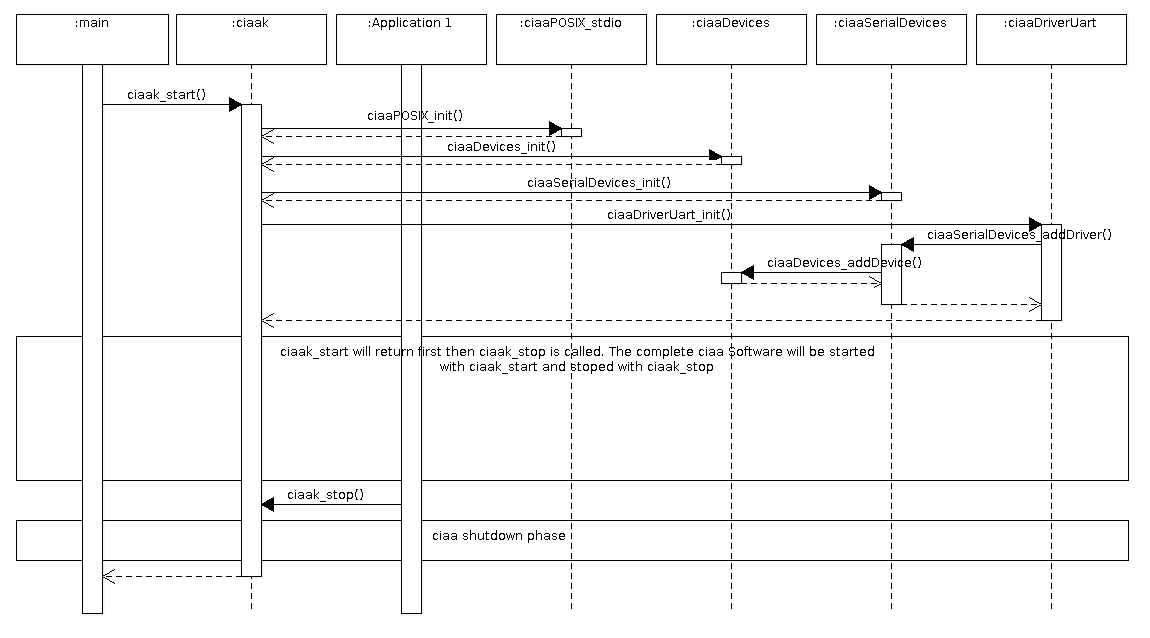
\includegraphics[height=5.5cm]{./Imagenes/lifecycle}
	\label{fig:lifcicle}
\end{figure}


\end{frame}
\section{Ejemplo}
\begin{frame}{POSIX Blinking}

\begin{center}
\textbf{Explore las potencialidades de la Juntura PN}
\end{center}
\begin{center}
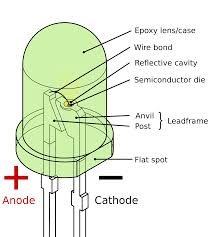
\includegraphics[height=5cm]{Imagenes/led}
\end{center}



\end{frame}

\end{document}


